\section{Leitungsbeläge}

\subsection{Elektrisches und magnetisches Feld}
% 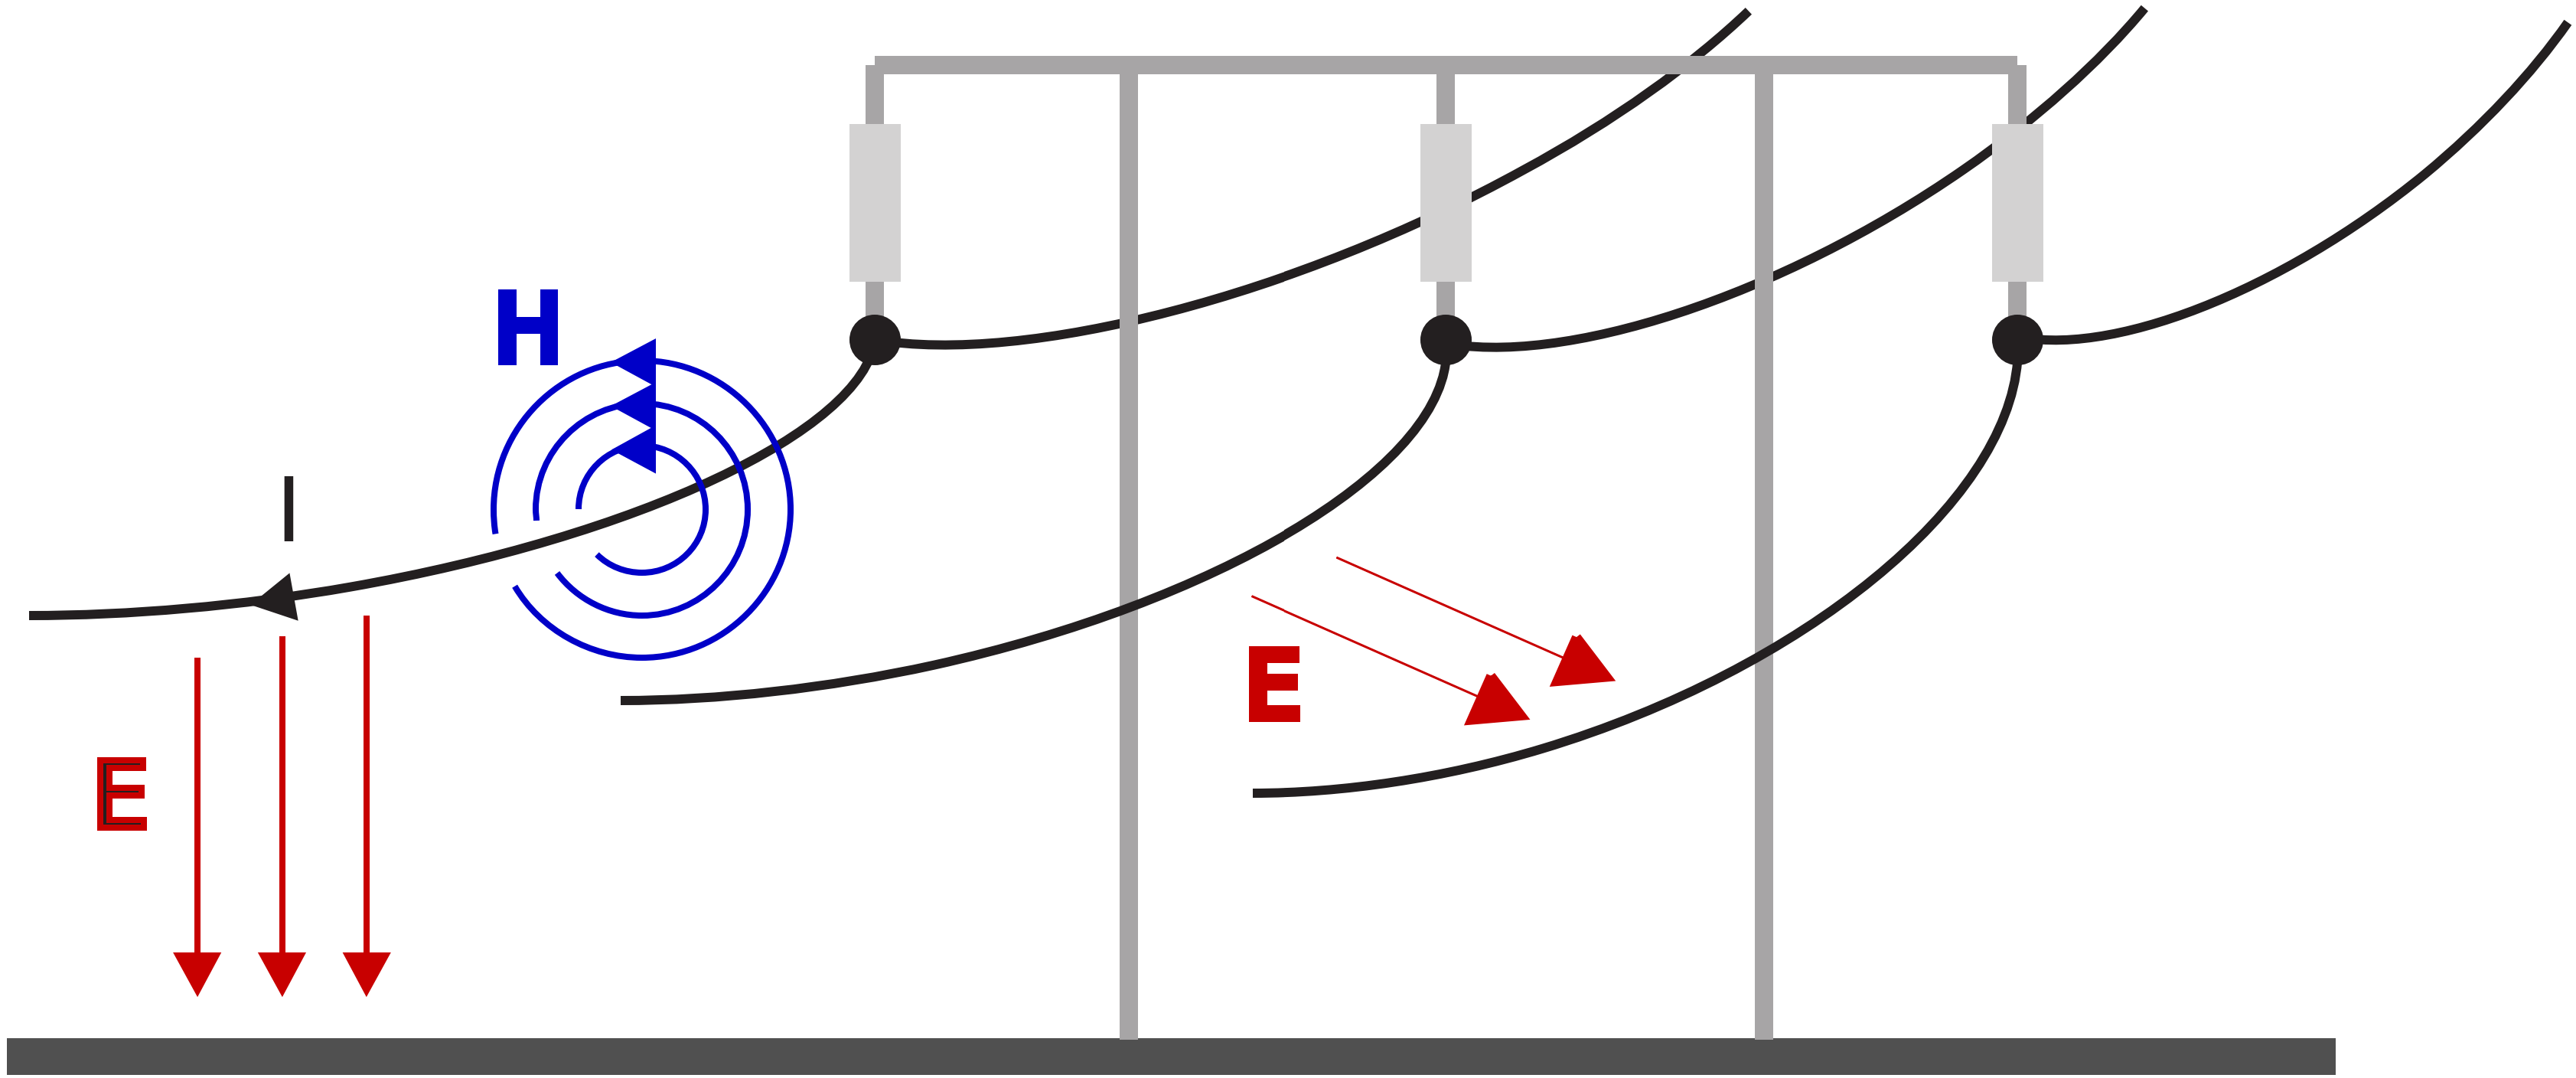
\includegraphics[width=0.98\columnwidth, align=c]{images/Elektrisches_und_Magnetisches_Feld.png}

\subsubsection{Ersatzschaltbild}
    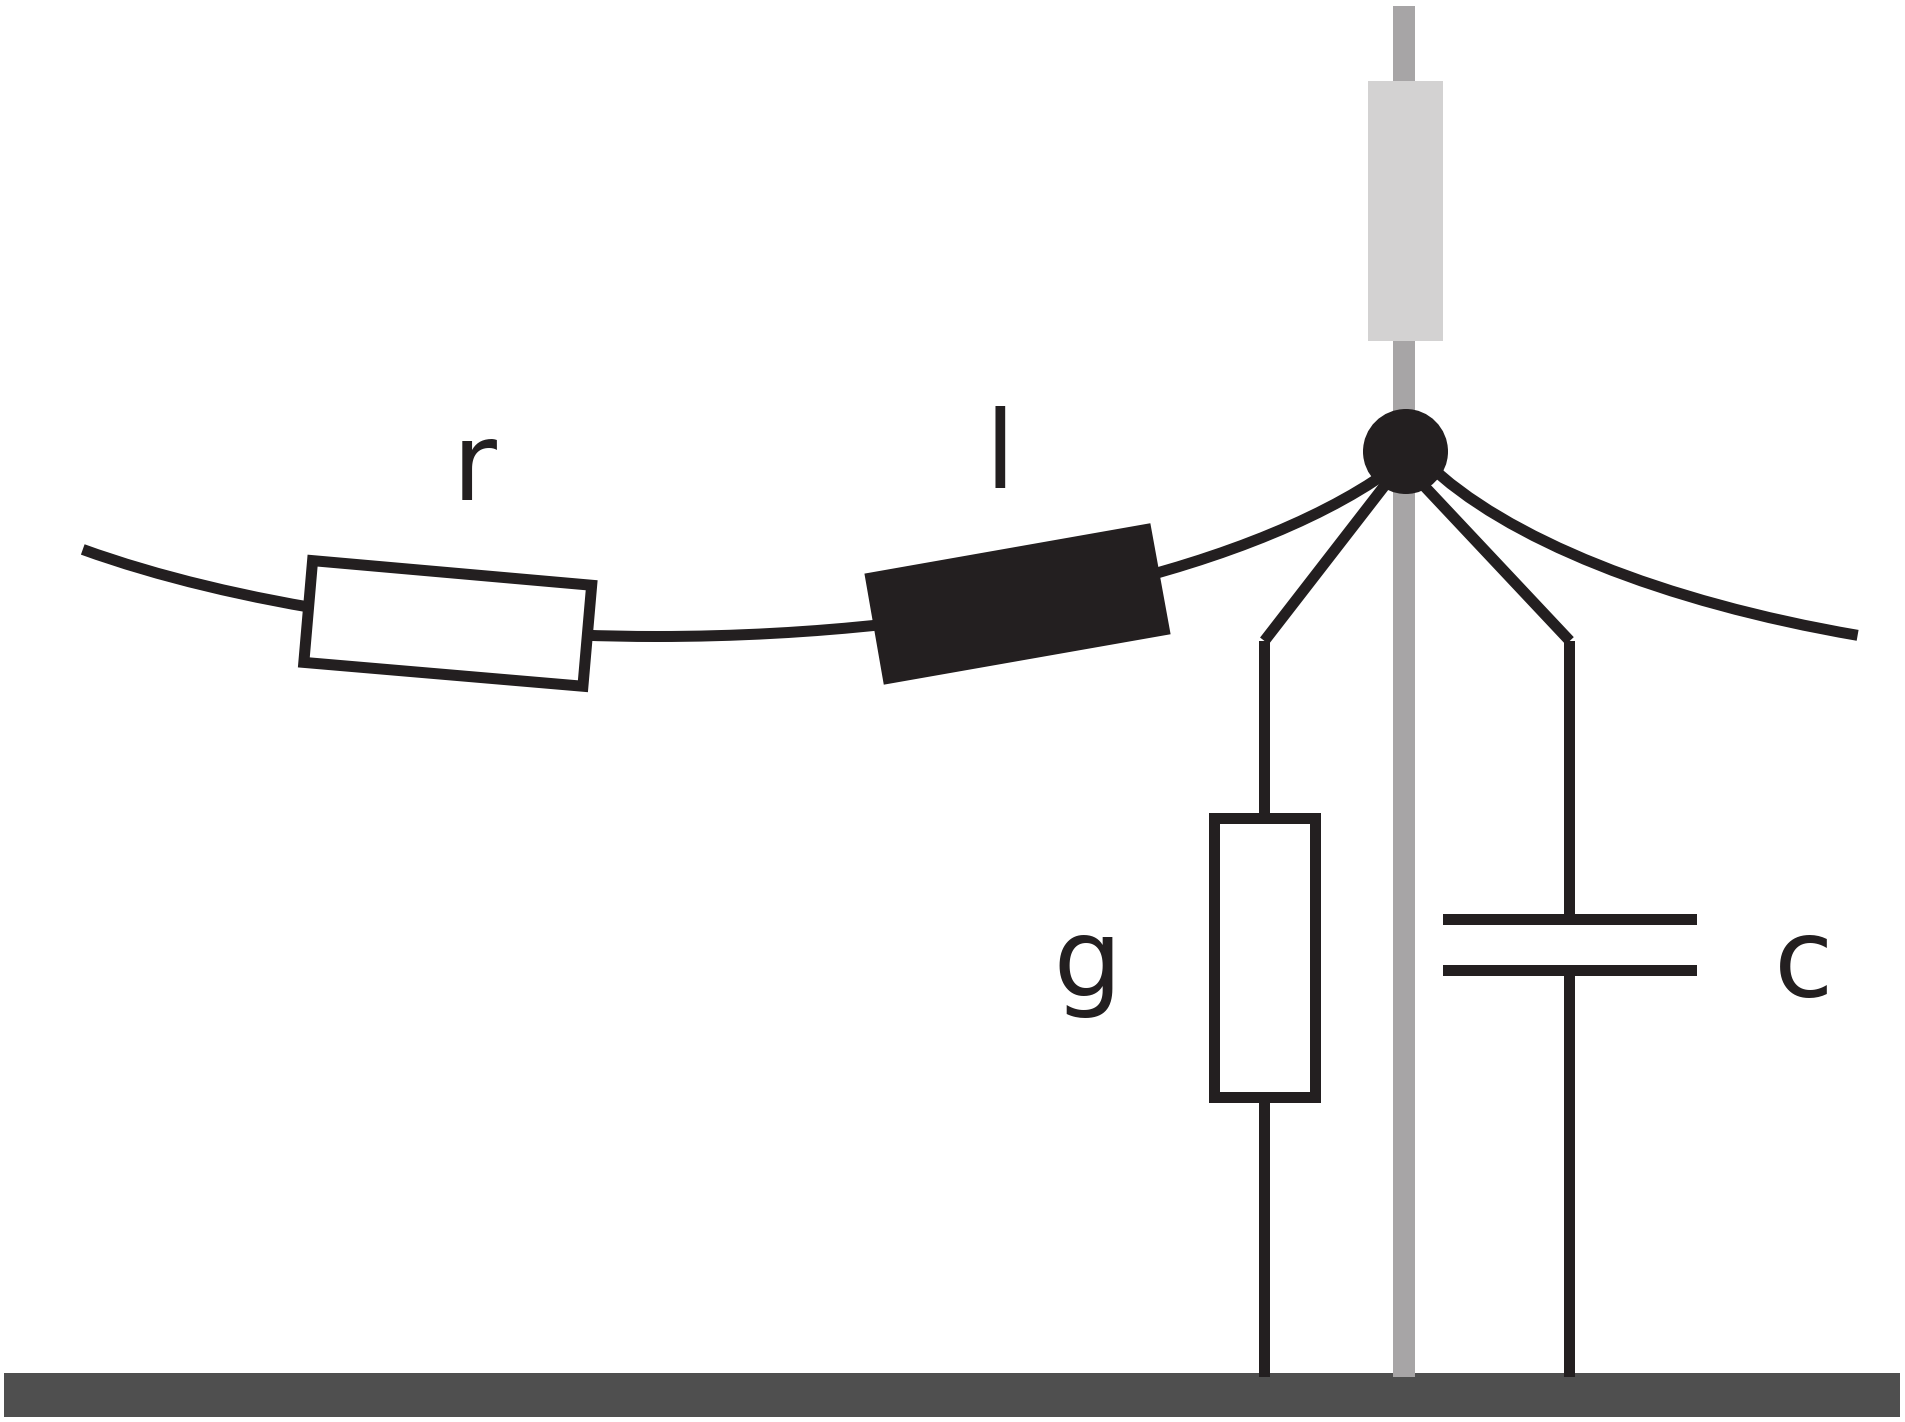
\includegraphics[width=0.7\columnwidth, align=c]{images/Ersatzschaltbild.png}
    \begin{minipage}[c]{0.3\columnwidth}
        \begin{itemize}
            \item Widerstandsbelag (r)
            \item Induktivitätsbelag (l)
            \item Ableitbelag (g)
            \item Kapazitätsbelag (c)
        \end{itemize}
    \end{minipage}


    \subsection{Widerstandsbelag r}
    % \newcolumn
    \subsubsection{Ursache}
    \begin{itemize}
        \item Ohmscher Widerstand des Leiterseils
        \item Bei \textbf{Wechselstrom} $\Rightarrow$ Berücksichtigung der \textbf{Stromverdrängung} (\textit{skin-effect})
    \end{itemize}


\subsubsection{Temperaturabhängigkeit des Widerstands}
    Der spezifische Widerstand $\rho$ ist temperaturabhängig und ergibt sich aus:

    \vspace{0.15cm}

    \begin{minipage}[t]{0.33\columnwidth}
        $
        \boxed{
        \rho = \rho_{\qty{20}{\degree}} \cdot \left[ 1 + \alpha \cdot \left(T - \qty{20}{\degree}\right) \right]
        }
        $ 
    \end{minipage}%
    \hfill
    \begin{minipage}[t]{0.65\columnwidth}
        \renewcommand{\arraystretch}{1.2}
        \begin{tabular}{l l l}
            $[\rho]$                    & Spezifischer Widerstand \dotfill                                & $\unit[per-mode=fraction]{\ohm\milli\metre\squared\per\metre}$ \\
            $[\rho_{\qty{20}{\degree}}]$& Spezifischer Widerstand bei $\qty{20}{\degreeCelsius}$ \dotfill & $\unit[per-mode=fraction]{\ohm\milli\metre\squared\per\metre}$ \\
            $[\alpha]$                  & Temperaturkoeffizient \dotfill                                  & $\unit[per-mode=fraction]{\per\degreeCelsius}$ \\
            $[T]$                       & Temperatur \dotfill                                             & $\unit{\degreeCelsius}$ \\
        \end{tabular}
    \end{minipage}

\subsubsection{Ohmscher Widerstand des Leiterseils}
    Der spezifische Widerstand $R'$ eines Leiterseils in $\frac{\Omega}{\text{m}}$ ergibt sich zu:

    \vspace{0.15cm}

    \begin{minipage}[t]{0.33\columnwidth}
        $
        \boxed{
        R' = \sigma \cdot \frac{\rho}{A}
        }
        $
    \end{minipage}%
    \hfill
    \begin{minipage}[t]{0.65\columnwidth}
        \renewcommand{\arraystretch}{1.2}
        \begin{tabular}{l l l}
            $[R']$      & Ohmscher Widerstand pro Meter \dotfill                & $\unit[per-mode=fraction]{\ohm\per\metre}$ \\
            $[\sigma]$  & Verseilfaktor (typisch $\sigma = 1{,}07$) \dotfill    & $-$ \\
            $[\rho]$    & Leitfähigkeit (spezifischer Widerstand) \dotfill      & $\unit[per-mode=fraction]{\ohm\milli\metre\squared\per\metre}$ \\
            $[A]$       & Leiterquerschnitt \dotfill                            & $\unit{\milli\metre\squared}$ \\
        \end{tabular}
    \end{minipage}

\subsection{Skin-Effekt}
    Die Eindringtiefe $\delta$ des elektrischen Feldes in einen Leiter ergibt sich zu:

    \vspace{0.15cm}

    \begin{minipage}[t]{0.33\columnwidth}
        $
        \boxed{
        \delta  = \sqrt{\frac{2 \cdot \rho}{\omega \cdot \mu}}
                = \sqrt{\frac{\rho}{\pi \cdot f \cdot \mu}}
        }
        $
    \end{minipage}%
    \hfill
    \begin{minipage}[t]{0.65\columnwidth}
        \renewcommand{\arraystretch}{1.2}
        \begin{tabular}{l l l}
            $[\delta]$   & Eindringtiefe des Stroms (Skin-Tiefe) \dotfill   & $\unit{\metre}$ \\
            $[\rho]$     & Spez. Widerstand des Leitermaterials \dotfill    & $\unit{\ohm\metre}$ \\
            $[\omega]$   & Kreisfrequenz \dotfill                           & $\unit[per-mode=fraction]{\radian\per\second}$ \\
            $[\mu]$      & Permeabilität des Leitermaterials \dotfill       & $\unit[per-mode=fraction]{\henry\per\metre}$ \\
        \end{tabular}
    \end{minipage}

    \vspace{0.1cm}

    \textit{\textbf{Bündelleiter} schwächen den Skin-Effekt durch die Aufspaltung des Querschnitts ab.}



\subsection{Ableitungsbelag g}
    \begin{itemize}
        \item Ensteht durch Verluste des Dielektrikums zwischen L-L und zwischen L-PE
        \item $G'$ ist sehr klein $\rightarrow$ bei norm. Betriebsverhältnissen gegenüber $\omega C'$ \textbf{vernachlässigbar}
        \item $G'$ ist grösser wenn Teilentladungen (Corona-Effekt) auftreten
        \item \textbf{Witterungsabhängig}
    \end{itemize}

\subsection{Induktivitätsbelag l}
    \begin{minipage}[t]{0.49\columnwidth}
        \begin{itemize}
            \item Entsteht durch Verkettung der magnetischen Flüsse
            \item Strom in L1 hat magnetische Flussverkettung zur Folge
            \item Fluss = verursachender Strom $\times$ Induktivität
        \end{itemize}
    \end{minipage}%
    \hfill
    \begin{minipage}[t]{0.49\columnwidth}
        \centering \vspace{-0.7\baselineskip}
        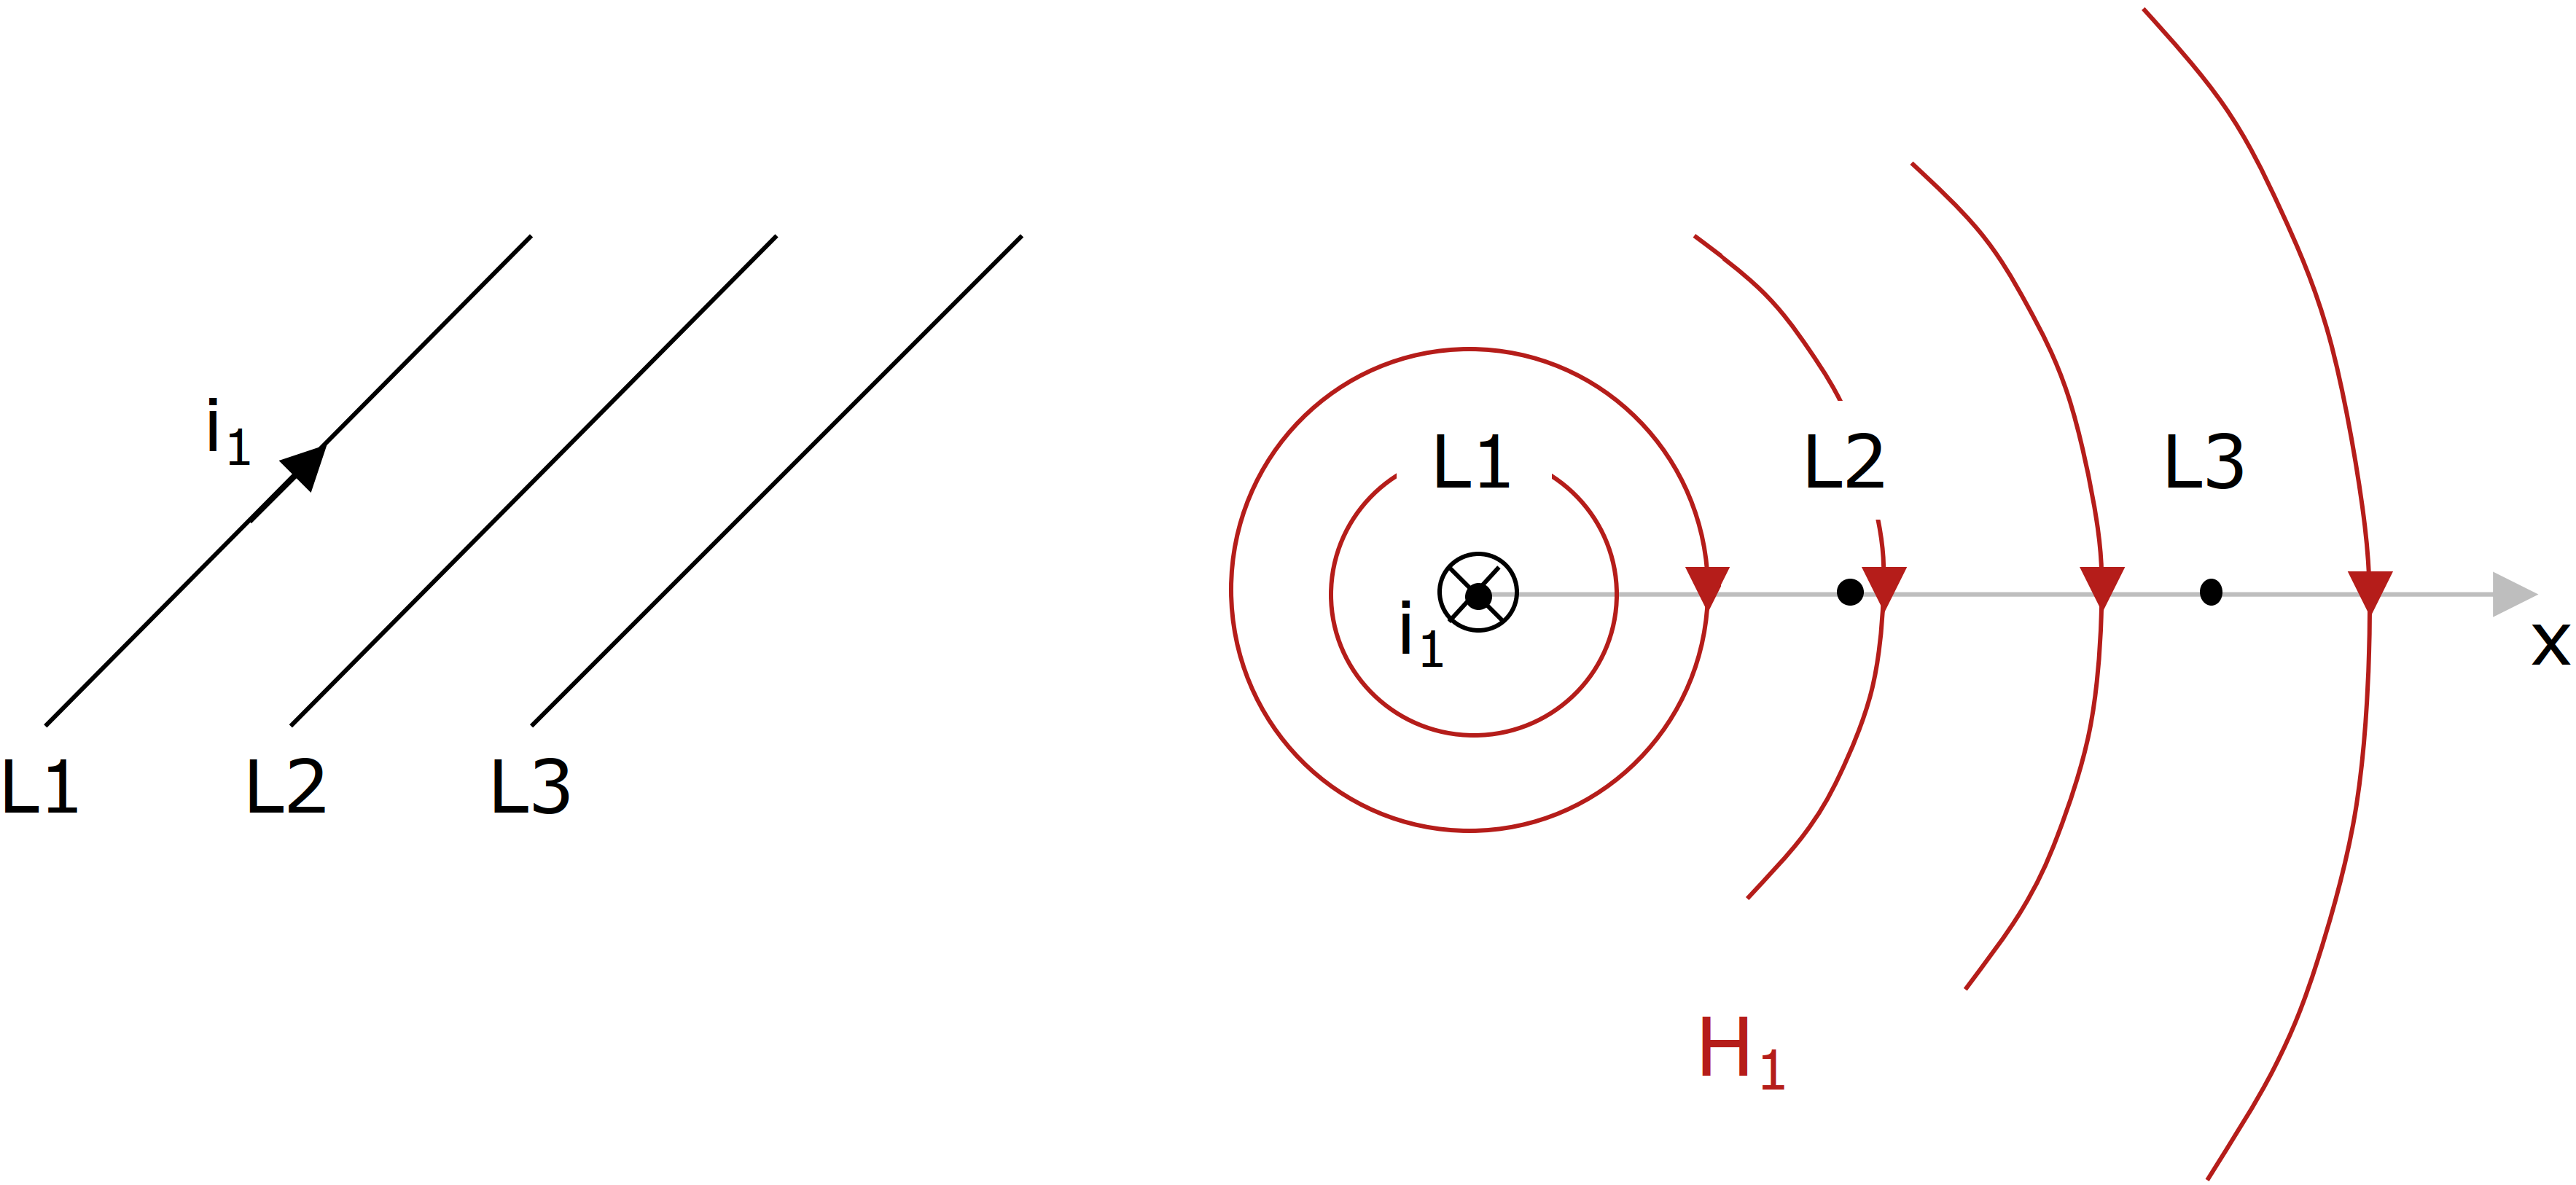
\includegraphics[width=0.9\columnwidth, align=c]{images/Induktivitätsbelag_1.png}
    \end{minipage}



\subsubsection{Herleitung}
    \begin{minipage}[t]{0.44\columnwidth}
        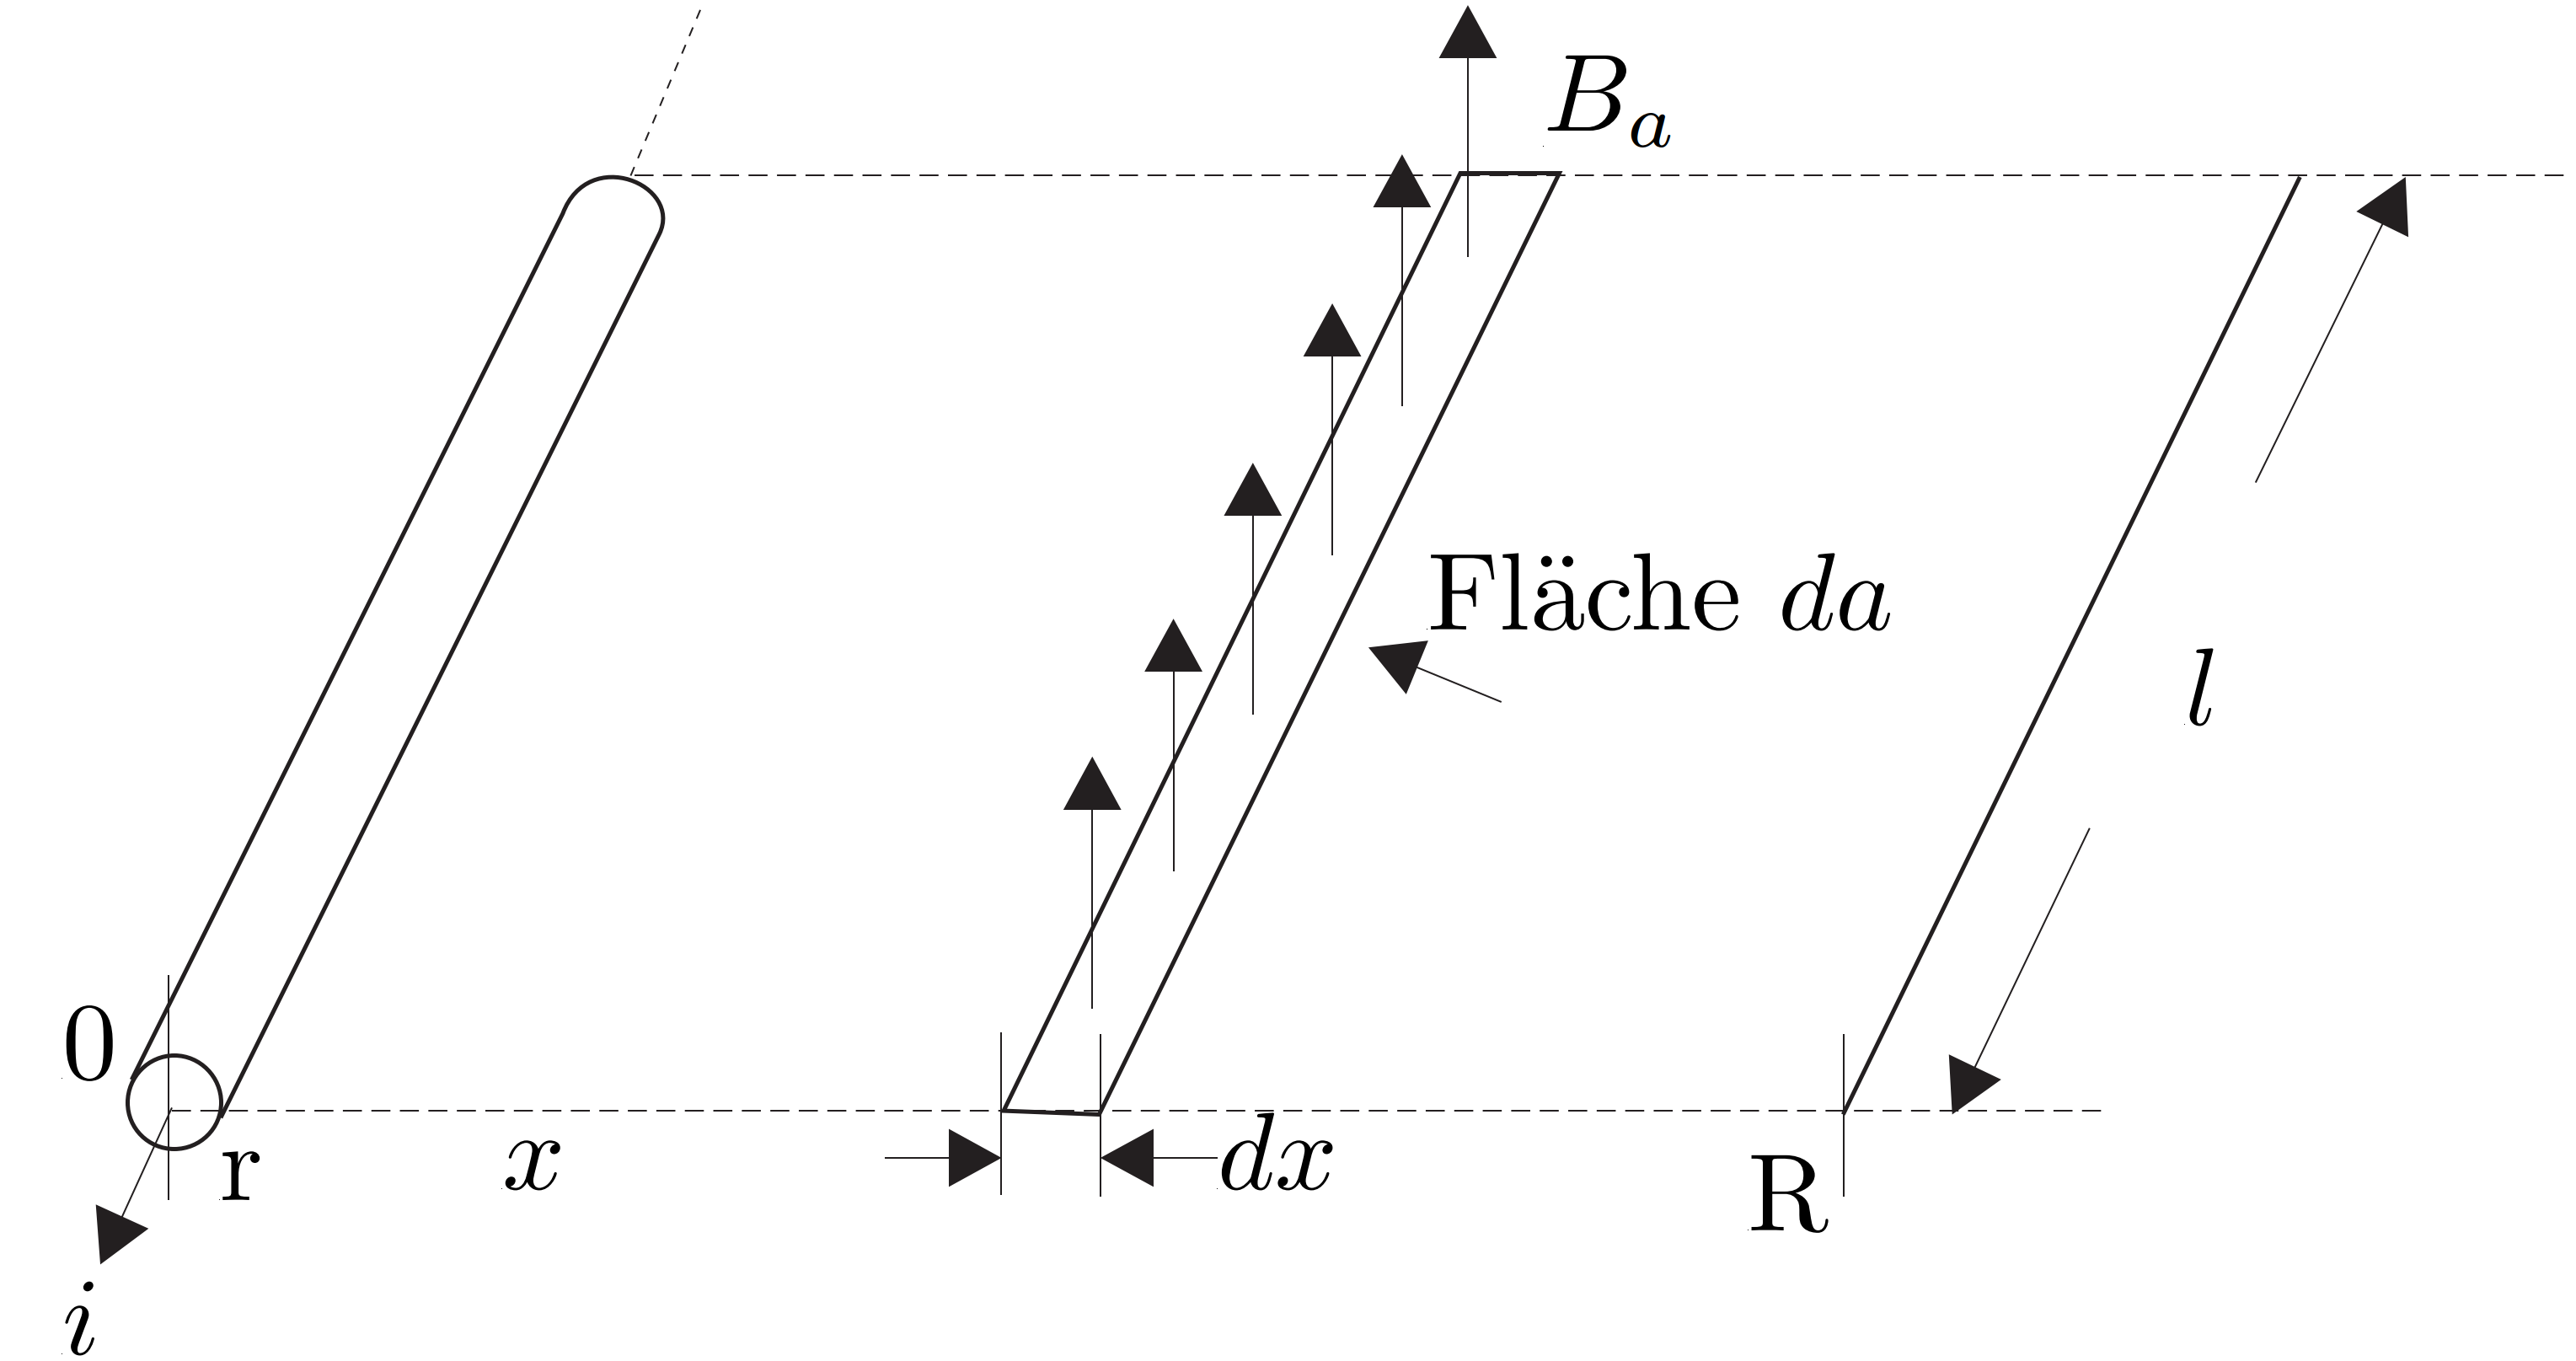
\includegraphics[width=0.9\columnwidth, align=c]{images/Induktivitätsbelag_2.png}
    \end{minipage}%
    \hfill
    \begin{minipage}[t]{0.55\columnwidth}
        $
        \begin{tabular}{rcl}
            $\phi_1$    &=& $\displaystyle \int_A B_1(x)\, da = \int_r^R B_1(x)\, dx$ \\
            $da$        &=& $l\, dx$ \\
            $B_1(x)$    &=& $\mu_0 H_1(x) \quad \text{and} \quad H_1(x) = \dfrac{i}{2\pi x}$ \\
            $\phi_1$    &=& $\mu_0 \displaystyle \int_r^R \frac{i}{2\pi x} \, l\, dx$ \\
                        &=& $\dfrac{\mu_0 i}{2\pi} \ln \dfrac{R}{r}$ \\
            $\phi_1$    &=& $L_1 i$ \\
            $L_1$       &=& $\dfrac{\mu_0}{2\pi} \ln \dfrac{R}{r}$
        \end{tabular}
        $
    \end{minipage}
\newcolumn

\subsubsection{Formel}
    Der Induktivitätsbelag $L'$ in $\unit[per-mode=symbol]{\henry\per\metre}$ enthält Eigeninduktivität und Kopplungsinduktivität\\
    Annahme: verdrillte Leitung, kreisförmiger Leiterquerschnitt

    \vspace{0.1cm}

    \begin{minipage}[t]{0.33\columnwidth}
        $
        \boxed{L' = \frac{\mu_0}{2 \cdot \pi} \cdot \ln\left( \frac{d}{0{,}78 \cdot r} \right)}
        $

        $
        \boxed{d = \sqrt[3]{d_{12} \cdot d_{23} \cdot d_{31}}}
        $
    \end{minipage}%
    \hfill
    \begin{minipage}[t]{0.65\columnwidth}
        \renewcommand{\arraystretch}{1.2}
        \begin{tabular}{l l l}
            $[L']$     & Induktivitätsbelag \dotfill                            & $\unit[per-mode=fraction]{\henry\per\metre}$ \\
            $[r]$      & Leiterradius \dotfill                                  & $\unit{\metre}$ \\
            $[d]$      & Mittlerer Leiterabstand \dotfill                       & $\unit{\metre}$ \\
            $[d_{ij}]$ & Abstand zwischen Phase $i$ und $j$ \dotfill            & $\unit{\metre}$ \\
            $[\mu_0]$  & Magnetische Feldkonstante $\num{4\pi e-7}$ \dotfill    & $\unit[per-mode=fraction]{\henry\per\metre}$ \\
        \end{tabular}
    \end{minipage}

    \vspace{0.1cm}

\subsubsection{Einfluss Leiterseilabstand auf Längsinduktivität}
    \begin{itemize}
        \item Grösserer Abstand erhöht die Induktivität, da der mag. Kopplungseffekt abnimmt
        \item Kleinere Abstände verringern die Längsinduktivität wegen stärkerer mag. Verkettung zwischen Phasenleitern
    \end{itemize}

    Der Abstand zwischen den Phasen (Leitern) wird von Zentrum zu Zentrum gemessen.

\subsection{Kapazitätsbelag c}
    Verursacht durch Kap. gegenüber anderen Aussenleitern sowie der Umwelt (Mast/Boden)

    \vspace{0.1cm}

    \begin{minipage}[t]{0.33\columnwidth}
        $ \boxed{C' = \frac{2 \pi k}{\ln\left(\frac{d}{r}\right)}}$
    \end{minipage}%
    \hfill
    \begin{minipage}[t]{0.65\columnwidth}
        \renewcommand{\arraystretch}{1.2}
        \begin{tabular}{l l l}
            $[C']$     & Kapazitätsbelag \dotfill                       & $\unit[per-mode=fraction]{\farad\per\metre}$ \\
            $[k]$      & Geometriefaktor \dotfill                       & $-$ \\
                       & (abh. z.\,B. von Masthöhe, Durchhang) \dotfill & \\
            $[d]$      & Mittlerer Leiterabstand \dotfill               & $\unit{\metre}$ \\
            $[r]$      & Leiterradius \dotfill                          & $\unit{\metre}$ \\
        \end{tabular}
    \end{minipage}

    \vspace{0.1cm}

    %     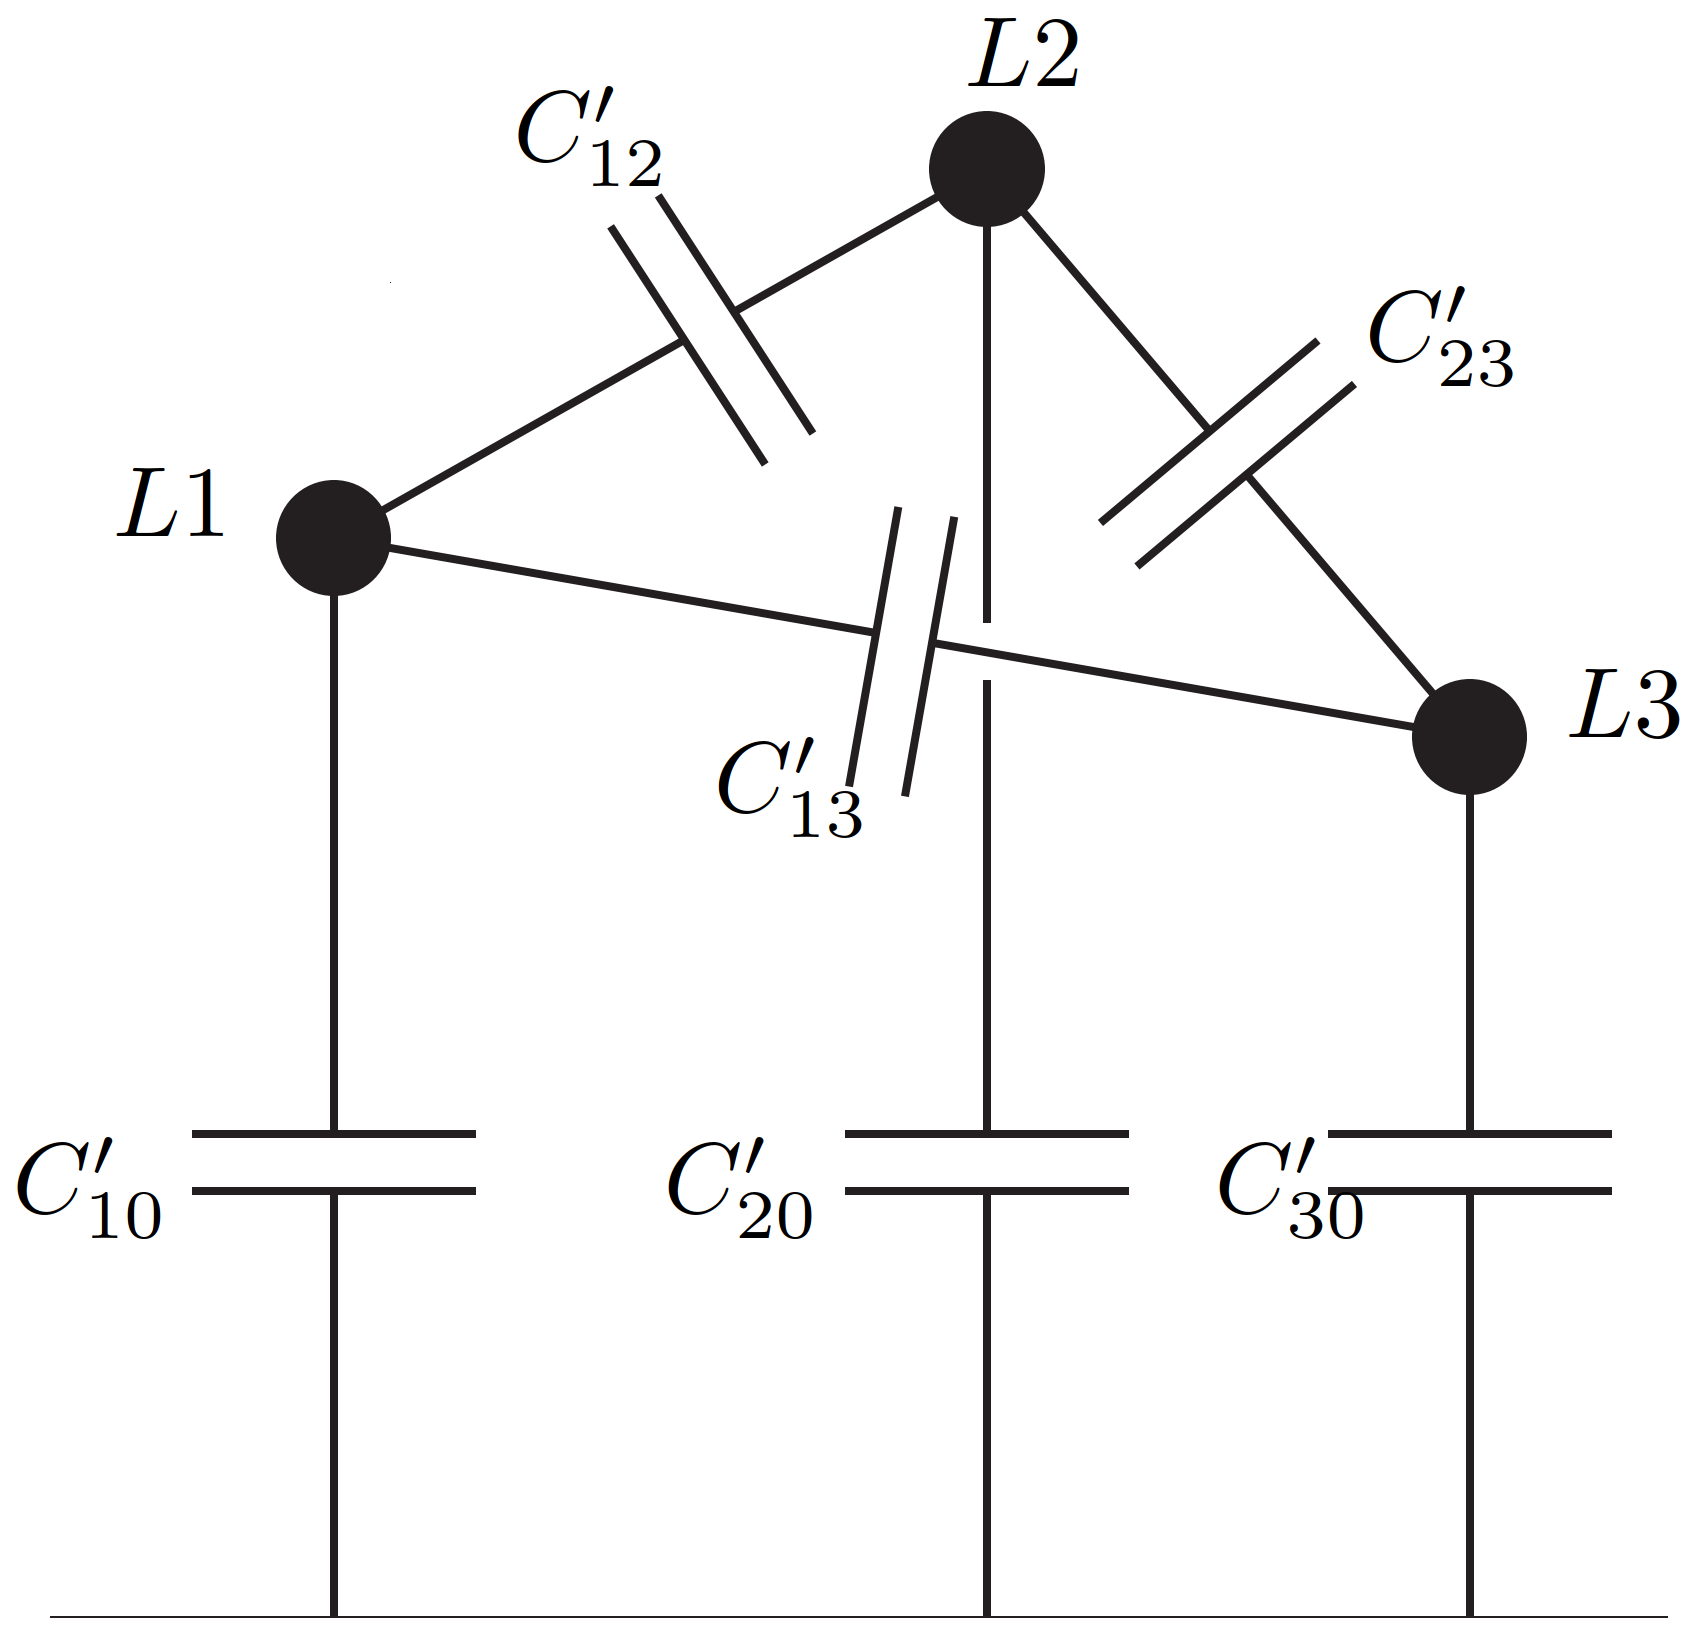
\includegraphics[width=0.35\columnwidth, align=c]{images/Kapazitätsbelag_1.png}

\subsection{Verdrillung}
    \begin{center}
        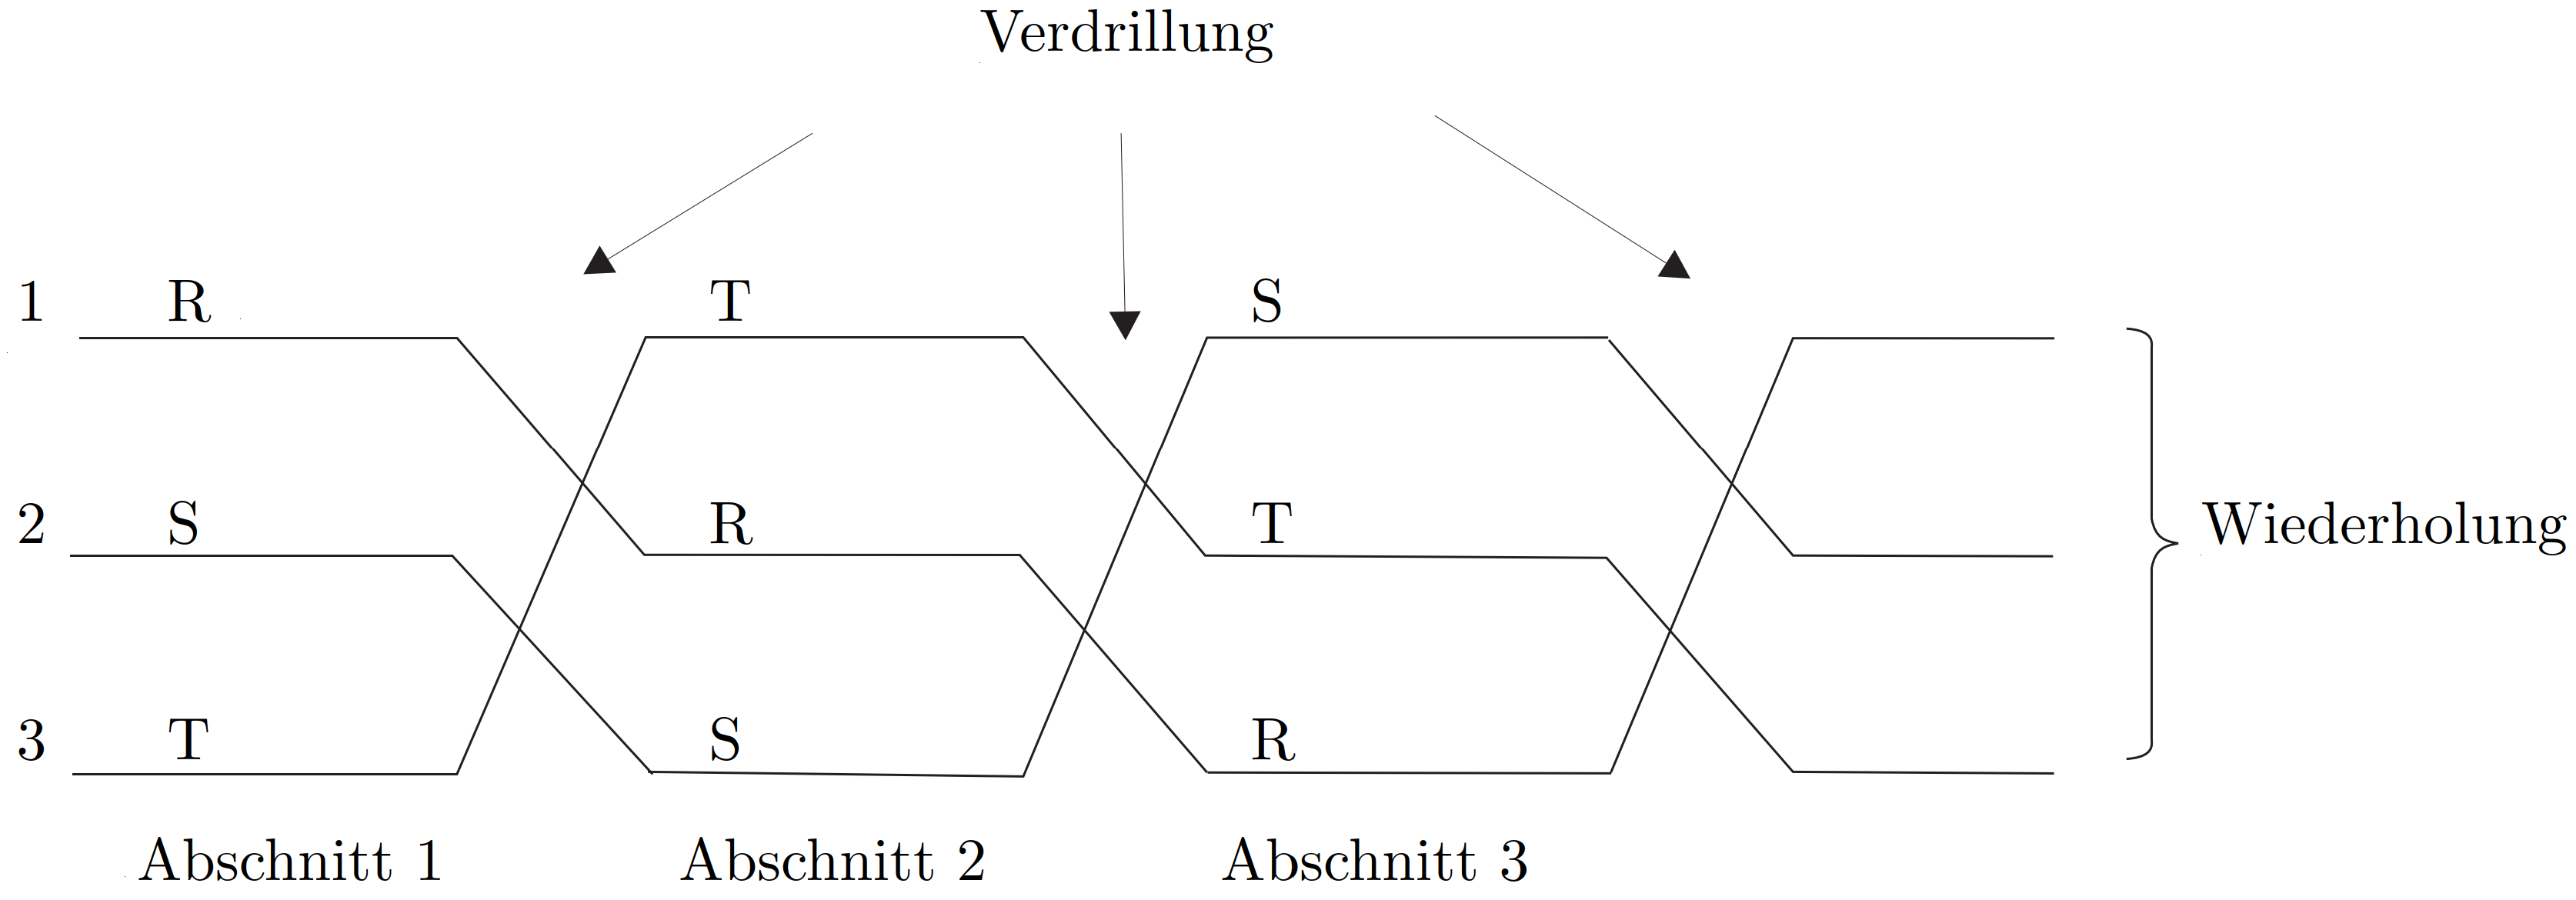
\includegraphics[width=0.9\columnwidth, align=c]{images/Verdrillung.png}
    \end{center}

    % \vspace{0.15cm}

    \begin{itemize}
        \item Die Leiterabstände sind bei einer Freileitung in der Regel nicht alle gleich.
        \item In Bezug auf die Koppelinduktivität ist die Leitung dann nicht symmetrisch.
        \item Man kann sie aber durch Phasentausch nach je einem Drittel der Leitungslänge symmetrisieren (verdrillen).
    \end{itemize}

\subsection{Bündelleiter}
    \begin{center}
        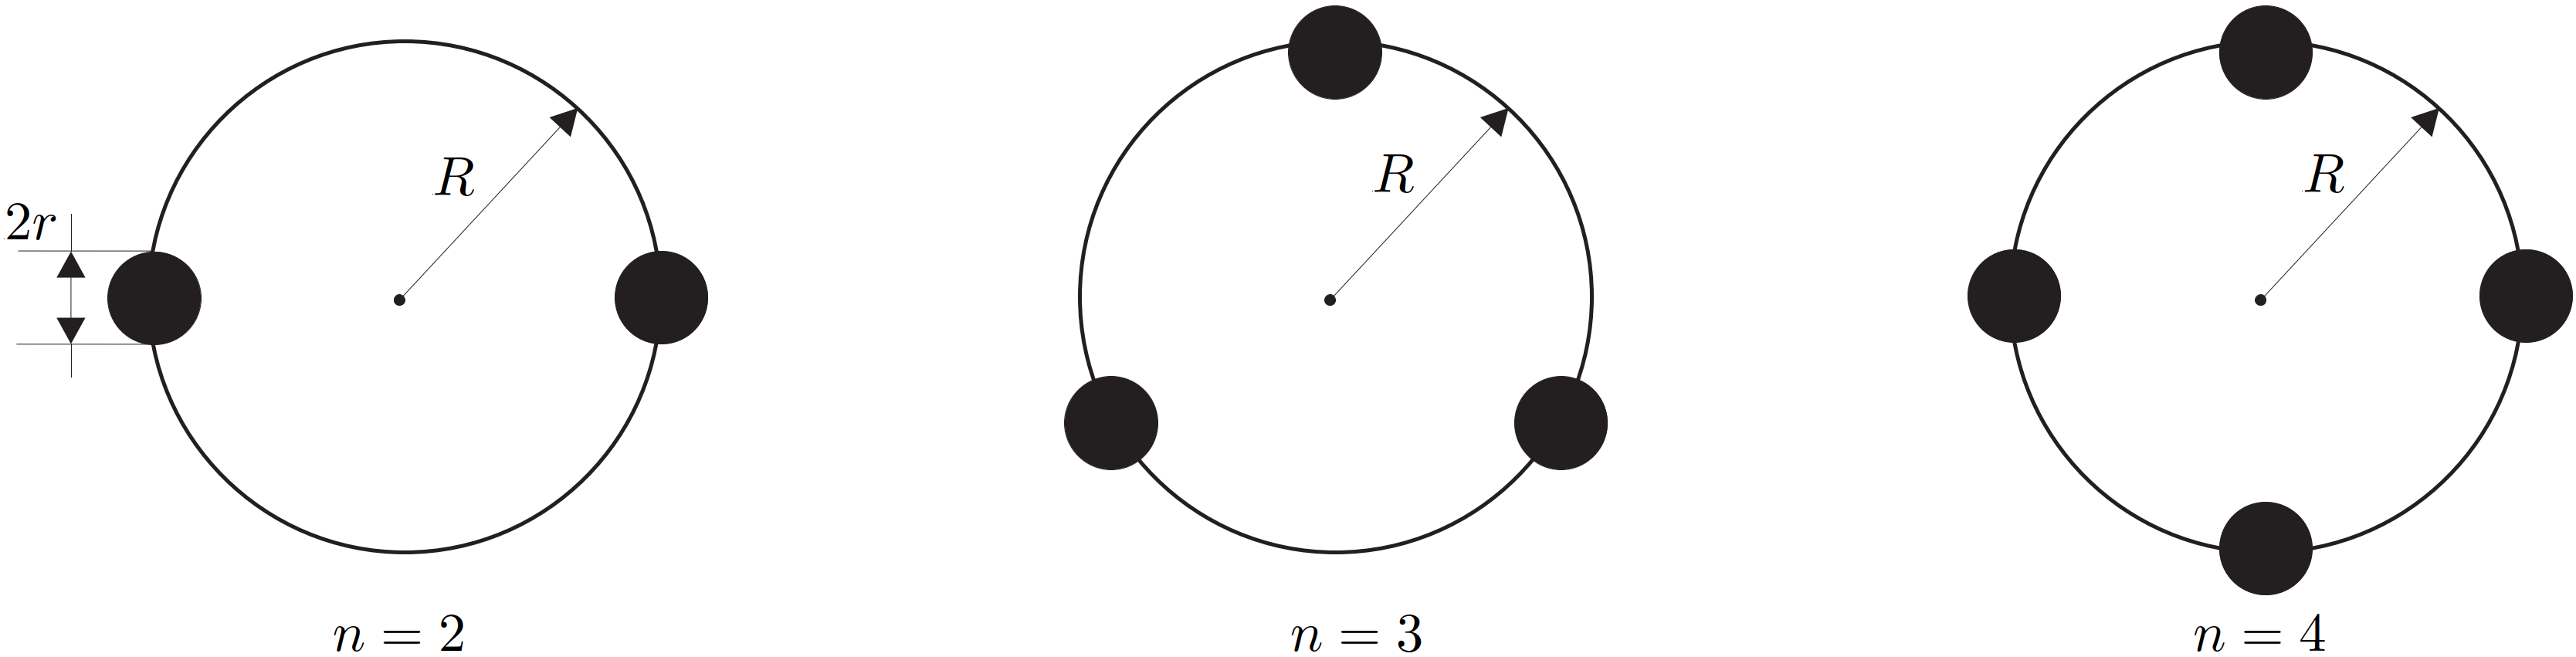
\includegraphics[width=0.98\columnwidth, align=c]{images/Bündelleiter.png}
    \end{center}

    \vspace{0.1cm}

    \begin{minipage}[t]{0.33\columnwidth}
        $ \boxed{r_\text{eq} = \sqrt[n]{n \cdot R^{(n-1)} \cdot r}} $
    \end{minipage}%
    \hfill
    \begin{minipage}[t]{0.65\columnwidth}
        \renewcommand{\arraystretch}{1.2}
        \begin{tabular}{l l l}
            $[r_\text{eq}]$ & Äquivalenter Leiterradius \dotfill                & $\unit{\metre}$ \\
            $[R]$           & Kreisradius der Bündelleiteranordnung \dotfill    & $\unit{\metre}$ \\
            $[r]$           & Teilleiterradius \dotfill                         & $\unit{\metre}$ \\
            $[n]$           & Anzahl der Bündelleiter \dotfill                  & $-$ \\
        \end{tabular}
    \end{minipage}

    \vspace{0.1cm}
